\section{Auswertung}
\label{sec:Auswertung}

Im ersten Schritt soll an den Detektor-Scan eine Gaußverteilung gefittet werden und der Wert der maximalen Intensität und der Halbwertsbreite sollen ermittelt werden.
Die Daten und der Fit sind in \ref{abb:detector} zu sehen.
Die Werte, die sich aus dem Fit ergeben haben sind 
\begin{align*}
a &= \num{1.815(15)e5} \\
\theta_0 &= \SI{0.0018(4)}{\degree} \\
\sigma &= \SI{0.0418(4)}{\degree}. \\
\end{align*}

Die Amplitude ergibt sich somit zu \num{1.732(22)e6} Events als Maximum. 
Die Halbwertsbreite beträgt $2 \sqrt{2 \ln 2} \sigma$ also \SI{0.0985(9)}{\degree}.
\begin{figure}
    \centering
    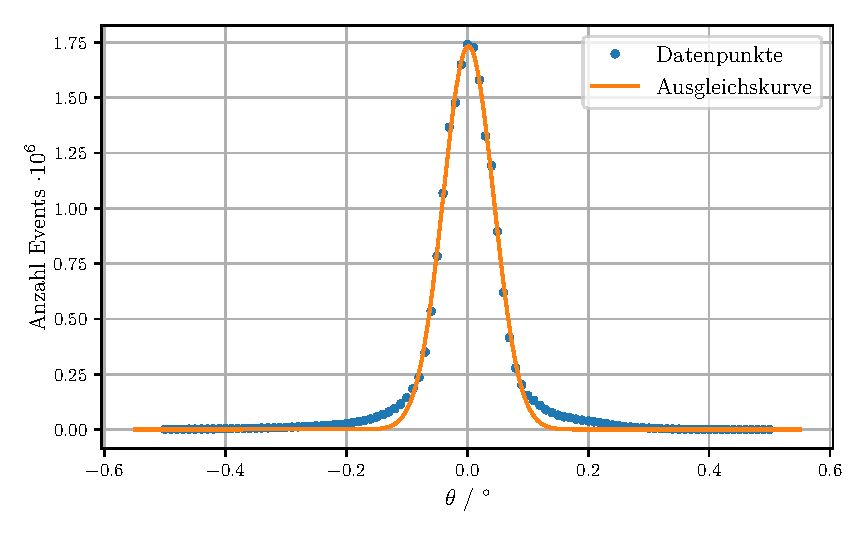
\includegraphics[width=\textwidth]{figures/detector_scan.pdf}
    \caption{Die gemessenen Daten des Detektor-Scans und eine an die Daten gefittete Gaußverteilung sind hier abgebildet.}
    \label{abb:detector}
\end{figure}

Die Reflektivität ergibt sich durch die Differenz aus dem diffusen Scan und den eigentlichen Messwerten. Die korrigierten Werte sind gemeinsam mit dem diffusen Scan und den Messwerten in \ref{abb:diffus} zu sehen.

\begin{figure}
    \centering
    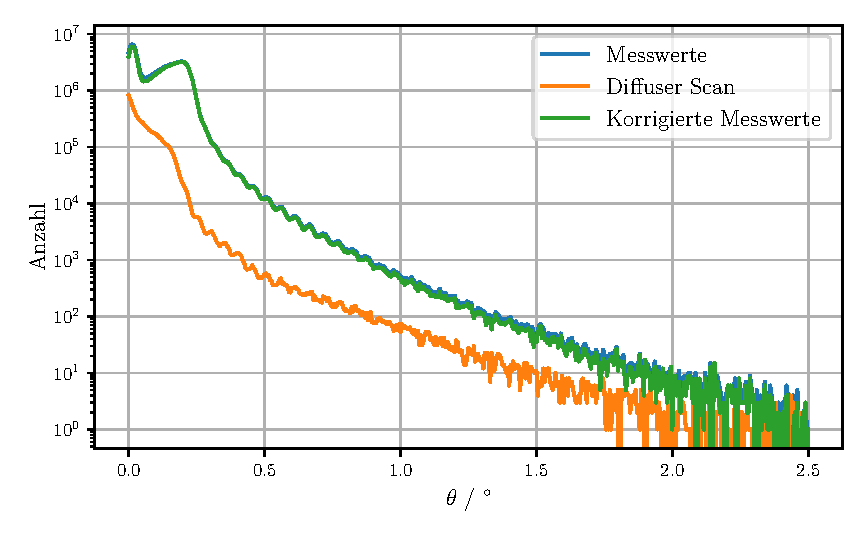
\includegraphics[width=\textwidth]{figures/messwerte_relativ.pdf}
    \caption{Die korrigierten Werte sind hier gezeigt, die sich als Differenz aus den Messwerten und dem diffusen Scan ergeben.}
    \label{abb:diffus}
\end{figure}

Dann werden die Werte am Winkel des Maximums \SI{0.195}{\degree} normiert und neben der Theoriekurve der Fresnelreflektivität einer idealen glatten Siliziumoberfläche, die sich aus Formel \eqref{eq:r} ergibt, in Abbildung \ref{abb:norm} aufgetragen. Der dafür benötigte Wellenvektor ergibt sich dabei über die Wellenlänge $\lambda = \SI{1.54e-10}{\meter}$ der K-$\alpha$ Linie von Kupfer. 
Der Brechungsindex von Silizium ist außerdem $n = \num{1} - \num{7.6e-6} + \num{1.73i e-9}$.
\begin{figure}
    \centering
    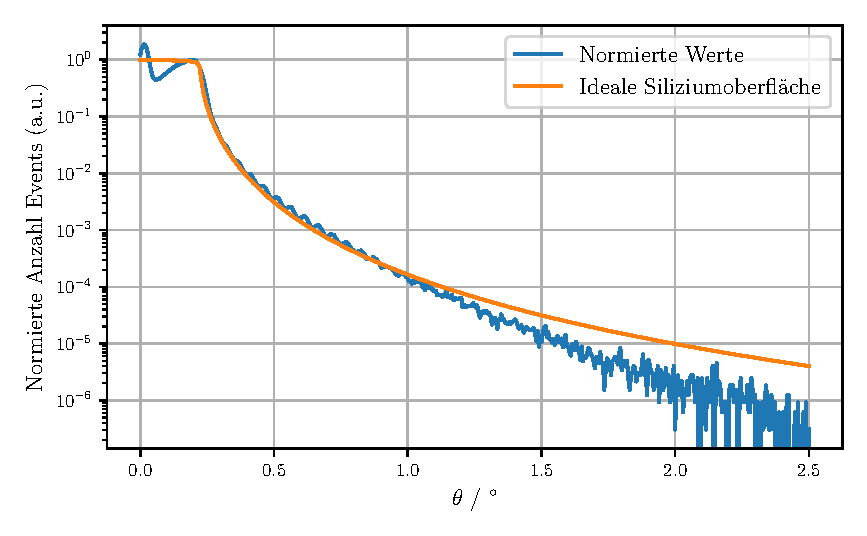
\includegraphics[width=\textwidth]{figures/messwerte_norm.pdf}
    \caption{Normierte Messwerte und die Theoriekurve der Fresnelreflektivität einer glatten Siliziumoberfläche.}
    \label{abb:norm}
\end{figure}

Der Geometriewinkel lässt sich aus der Abbildung \ref{abb:dreieck} ablesen. Der Abstand von der Mitte zu den Schnittpunkten des Dreiecks entspricht dem Wert des Geometriewinkels. Dieser beträgt \SI{0.72}{\degree}. Mithilfe der Formel \eqref{eq:geometrie} und dem gemessenen Durchmesser der Probe, der $D = \SI{2}{\milli\metre}$ beträgt, ergibt sich ein Geometriefaktor von $G = \num{80} \cdot \sin \alpha_i$.

\begin{figure}
    \centering
    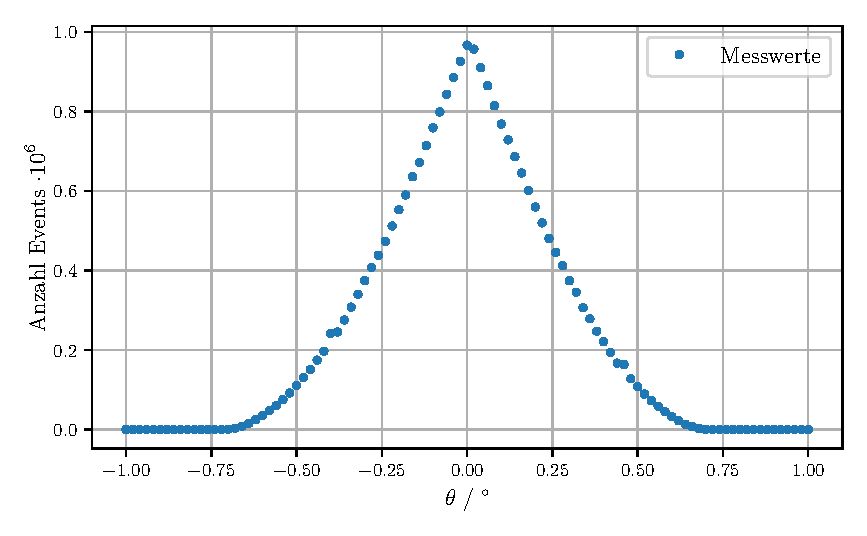
\includegraphics[width=\textwidth]{figures/dreieck.pdf}
    \caption{Hier sind die Messwerte des Rocking-Scan während der Justage aufgetragen.}
    \label{abb:dreieck}
\end{figure}

Aus den Kiessig Oszillationen ergibt sich nach Gleichung \eqref{eq:kiessig} die Schichtdicke. 
Dafür müssen die Stellen der Minima bestimmt werden. Hier wurden 8 eindeutige Minima gemessen. Aus den Positionen dieser Minima lässt sich dann der Betrag der $q$-Werte bestimmen und aus der Differenz dieser Werte ergibt sich dann die Schichtdicke. Diese beträgt im Mittel $z = \SI{900(40)}{\angstrom}$. 

Zur Bestimmung des Dispersionsprofils wird der Parratt-Algorithmus benutzt. 
In Abbildung \ref{abb:parratt} sind die Messwerte zusammen mit einer Theoriekure des Parratt-Algorithmus aufgetragen. 
Als Parameter wurden hierbei nach Formel \eqref{eq:imag} und \eqref{eq:rau} die Werte 
\begin{align*}
 \delta_\text{Si} &= \num{5.7e-6}\\
 \delta_\text{PS} &= \num{5.1e-6} \\
 \beta_\text{Si} &= \num{6.13e-7}\\
 \beta_\text{PS} &= \num{4.9e-7} \\
 \sigma_\text{Si} &= \num{8e-10} \\
 \sigma_\text{PS} &= \num{5.5e-10}. \\
\end{align*}

\begin{figure}
    \centering
    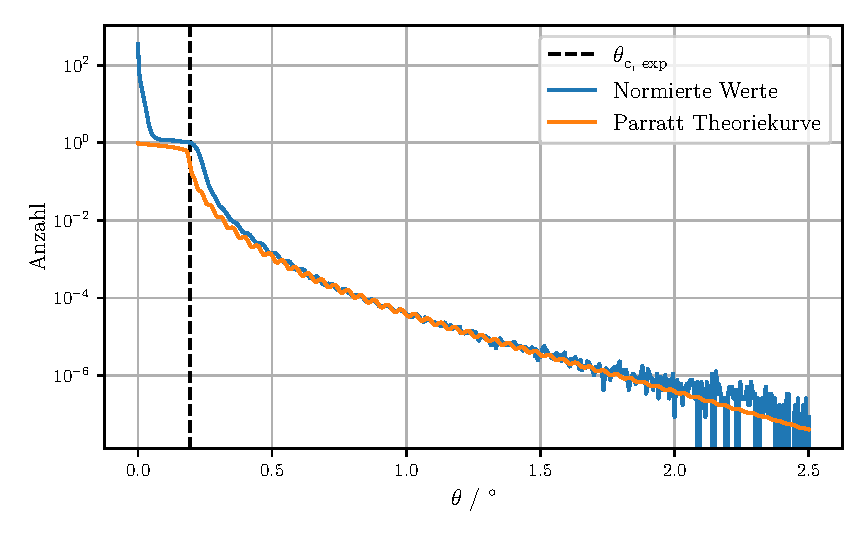
\includegraphics[width=\textwidth]{figures/parat.pdf}
    \caption{Hier sind die Messwerte und eine Theoriekurve des Parratt-Algorithmus.}
    \label{abb:parratt}
\end{figure}

Aufgrund der Formel \eqref{eq:delta} ergibt sich aus den $\delta$-Werten der Theoriekurve ein kritischer Winkel von $a_\text{c, Si}= \SI{0.19}{\degree}$ und $a\_text{c, PS}= \SI{0.18}{\degree}.$

